\documentclass[]{Liebert_Author_revised}
\usepackage[T1]{fontenc}
\usepackage[utf8]{inputenc}
\usepackage{lmodern}
\usepackage{bm}
\usepackage{epstopdf}
\usepackage{float}
\usepackage{tabularx}
\usepackage[margin=1in]{geometry}
\usepackage{caption}
\captionsetup{font={normalsize,doublespacing}}
\AddToHook{env/table/begin}{\doublespacing}
\hypersetup{hidelinks}
\setcitestyle{aysep={}}
\setlength{\emergencystretch}{2em}
\raggedbottom
\widowpenalty=10000
\clubpenalty=10000

\title{Fused Lasso Improves Accuracy of Co-occurrence Network Inference in Grouped Samples}

\author{\parbox{\dimexpr\textwidth-2\tabcolsep\relax}{\centering Daniel Agyapong,$^{1\ast}$ Briana H. Beatty,$^{2}$ Peter G. Kennedy,$^{2}$\\ 
Jane C. Marks,$^{3}$ Toby D. Hocking$^{4}$\\
{$^{1}$School of Informatics, Computing, and Cyber Systems, Northern Arizona University,}\\
{Flagstaff, Arizona, United States of America}\\
{$^{2}$Department of Plant and Microbial Biology, University of Minnesota,}\\
{Saint Paul, Minnesota, United States of America}\\
{$^{3}$Department of Biological Sciences, Northern Arizona University,}\\
{Flagstaff, Arizona, United States of America}\\
{$^{4}$Département d'informatique, Université de Sherbrooke,}\\
{Quebec, Canada}\\
{$^\ast$To whom correspondence should be addressed;}\\
{E-mail: da2343@nau.edu.}}
}

\date{}

\begin{document}

\maketitle

\begin{abstract}
Co-occurrence network inference algorithms have significantly advanced our understanding of microbiome communities. Microbiome network inference often analyzes groups independently or pools all samples, limiting the ability to share information while retaining differences between environments.

We evaluated separate, pooled, and fused lasso models on grouped microbiome datasets using Same-All Cross-validation (SAC). Models were trained using samples from the group being tested (Same) or from all groups (All), with predictions evaluated on samples excluded from training. The fused models share information through a penalty on differences between regression coefficients across groups.

Our results demonstrate that fusion improved predictive performance across grouped datasets, although the preferred model varied among taxa. After log ratio transformation, the benefit over separate models was broadly maintained, while the advantage over a pooled model depended on the dataset and preprocessing.

SAC provides a framework for evaluating whether sharing information across groups improves prediction. SAC helps biologists assess whether combining information across related groups improves prediction when collecting additional samples is costly.
\end{abstract}
\keywords{microbiome; temporal dynamics; multi-algorithm analysis; microbial ecology}

\section{Introduction}
Microbial communities represent complex ecological systems where numerous species interact in complex networks that influence its structure and function.
Co-occurrence network inference algorithms have emerged as important tools for explaining these interactions, helping researchers understand the complex dynamics of microbiome associations in different environments \citep{faust2012microbial,lima2015determinants}.
Despite significant advances in microbial network analysis, there has been limited exploration of how microbial communities adapt and form associations across changing environments \citep{baldo2017convergence}.
Most existing research has focused on characterizing microbiome networks within single habitats or combined different environmental samples without preserving their ecological distinctions \citep{weiss2016correlation}.

Several methods address compositionality in microbiome network inference.
SparCC and CCLasso estimate latent correlation structure \citep{friedman2012sparcc,fang2015cclasso}, SPIEC-EASI estimates sparse conditional dependence networks after compositional transformation \citep{Kurtz2015}, and mLDM uses a hierarchical lognormal-Dirichlet-multinomial model to estimate microbial and environmental associations \citep{yang2017mldm}.
These methods differ in their assumptions and in the statistical networks they estimate.

Traditional algorithms often assume the same model parameters (e.g., regression weights, network edge strengths) apply equally whether working with combined data or with each dataset separately, neglecting their potential inter-dependencies and thus failing to capture distinct ecological dynamics of individual environments \citep{knights2011bayesian,marcos2021applications}.

This limitation becomes increasingly problematic when trying to predict microbiome associations across diverse environments, as these approaches ignore the ecological factors that shape community structures in different habitats \citep{costello2012application}.
Recent methodological advances by \citet{agyapong2025cross} have addressed some of these challenges through the introduction of novel cross-validation methods for training and testing co-occurrence network inference algorithms, providing a more robust framework for evaluating network quality for various algorithms.
Our study addresses this critical gap by investigating the spatial and temporal dynamics of microbial communities through the cross-validation analysis of grouped samples across diverse environments.

Using publicly available microbiome datasets collected from diverse habitats and at different times, we evaluate how well algorithms predict microbial associations when samples are pooled across environments versus kept separate (Same-All Cross-validation, SAC) \citep{thaiss2016microbiome,thompson2017}.
This framework allows us to better understand how environmental ecological factors influence microbial associations and community assembly.
We evaluate the traditional \texttt{glmnet} and \texttt{fuser}, which is a novel algorithm in the context of microbiome network inference that preserves information from each group during combined training, enabling it to generate distinct predictive networks for diverse environmental niches.
We refer to separate models trained within each group as \texttt{glmnet\_same}, one pooled model trained across groups as \texttt{glmnet\_all}, and models trained jointly with fusion across groups as \texttt{fuser\_all}.
We use \texttt{glmnet} as a direct comparator because both approaches use squared error loss and an L1 sparsity penalty for predicting individual taxa \citep{friedman2010glmnet,dondelinger2016hdlss}.
Comparing separate, pooled, and fused models under a common cross-validation framework allows us to assess whether sharing information through fusion improves predictive performance.
Unlike conventional approaches that apply uniform coefficients across combined datasets, \texttt{fuser} maintains contextual integrity while integrating data across environments \citep{papoutsoglou2023machine}.
Our approach builds upon recent cross-validation techniques introduced by \citet{agyapong2025cross} for inference algorithm evaluation, extending them to preserve the niches represented by each group during network generation.
The \texttt{fuser} algorithm not only achieves comparable performance to existing algorithms when trained and tested on homogeneous environmental groups but significantly outperforms baseline algorithms in predictions across groups \citep{moreno2021statistical}.
Our findings have important implications for understanding the ecological drivers of microbiome community assembly and for developing more accurate predictive models across heterogeneous environmental niches.

The fused graphical lasso estimates multiple precision matrices through a penalized Gaussian likelihood, encouraging corresponding entries to be similar across groups \citep{danaher2014joint}.
Our approach fits a neighborhood regression for each taxon and penalizes differences between corresponding regression coefficients across groups.
Neighborhood selection also connects regression to graphical model estimation: \citet{lin2017joint} use Bayesian neighborhood selection with a Markov random field prior to share network structure across groups.
Our contribution is the application and evaluation of fusion within the Same-All cross-validation framework for grouped microbiome samples.

\section{Microbiome Datasets}
We collected publicly available microbiome datasets containing grouped samples from human microbiomes and soil decomposition experiments.
Table~\ref{tab:datasets} summarizes their biological origins and dataset characteristics; preprocessing and group balancing are described in the following section.

\begin{table}[t]
\centering
\caption{Microbiome datasets with grouped samples}
\label{tab:datasets}
\setlength{\tabcolsep}{4pt}
\begin{tabularx}{\textwidth}{@{}>{\raggedright\arraybackslash}X r r r r@{}}
\hline
Dataset and description & \shortstack{No. of\\Taxa} & \shortstack{No. of\\Samples} & \shortstack{No. of\\Groups} & \shortstack{Sparsity\\(\%)} \\
\hline
\textbf{HMPv13} \citep{HMP2012}. Healthy human microbiomes across multiple body sites. & 5,830 & 3,285 & 71 & 98.16 \\
\addlinespace[4pt]
\textbf{HMPv35} \citep{HMP2012,Huttenhower2012}. Human 16S profiles processed with QIIME at 97\% sequence similarity. & 10,730 & 6,000 & 152 & 98.71 \\
\addlinespace[4pt]
\textbf{MovingPictures} \citep{Caporaso2011}. Repeated sampling of multiple body sites in two individuals. & 22,765 & 1,967 & 6 & 97.06 \\
\addlinespace[4pt]
\textbf{qa10394} \citep{qa10394}. Human and canine faecal microbiomes under different storage preservatives and temperatures. & 9,719 & 1,418 & 16 & 94.28 \\
\addlinespace[4pt]
\textbf{TwinsUK} \citep{TwinsUK,Goodrich2016}. Twin 16S profiles for studying genetic and environmental effects. & 8,480 & 1,024 & 16 & 87.70 \\
\addlinespace[4pt]
\textbf{necromass}. Bacterial and fungal communities in Minnesota pine forest soils: high or low melanization at 1 or 3 months, plus soil controls. & 36 & 69 & 5 & 39.78 \\
\hline
\end{tabularx}
\end{table}

\section{Methodology}
\subsection{Preprocessing and Data Preparation}
We preprocessed the microbiome datasets to ensure balanced representation across experimental groups and to prepare the data for downstream machine learning analyses.
The preprocessing pipeline consisted of the following sequential steps:
We applied a log10 transformation with pseudocount addition ($\log_{10}(count + 1)$) to the raw OTU count data.
This transformation helps stabilize variance across different abundance levels and reduces the influence of highly abundant taxa while preserving zero values \citep{agyapong2025cross, weiss2017normalization}.
To ensure equal representation across experimental groups for cross-validation procedures, we balanced group sizes on the mean group size, excluding smaller groups and randomly subsampling the remaining groups without replacement.
This approach prevents group size imbalances from biasing downstream analyses \citep{Knights2011supervised, pasolli2016machine}.
We removed low-prevalence OTUs to reduce sparsity and potential noise in downstream models \citep{papoutsoglou2023machine,Cao2021,Kurtz2015}.
Finally, we ensured that the resulting datasets contained equal numbers of samples per experimental group, with log-transformed OTU abundances ready for machine learning model training and evaluation.


\subsection{Same All Cross-validation (SAC)}
Cross-validation (CV) is a fundamental technique in machine learning and statistical modeling used to assess how well a model predicts unseen observations \citep{stone1974cv,agyapong2025cross}.
This study introduces Same-All Cross-validation (SAC), a constrained variant of the Same/Other/All K-fold cross-validation (SOAK) framework originally proposed by Hocking et al. (2024) for measuring pattern similarity across data subsets \citep{hocking2024soaksameotherallkfoldcrossvalidation}.
Our Same-All Cross-validation (SAC) framework is designed to rigorously evaluate the performance and generalizability of microbiome network inference algorithms across groups.
SAC builds upon the principles of traditional cross-validation but introduces two distinct validation scenarios:

\begin{enumerate}
    \item \textbf{Same}: In this scenario, algorithms are trained and tested exclusively within the same group.
    This approach allows for a focused evaluation of how well algorithms can capture the specific interactions and relationships present in a given group.
    \citet{agyapong2025cross} utilized this CV scenario extensively on microbiome datasets, which is also used in traditional CV approaches.
    In this study, the Same scenario fits a separate model within each group, using distinct training and test samples from that group. We denote the separate glmnet models by \texttt{glmnet\_same}.

    \item \textbf{All}: In this scenario, algorithms are trained on data from all available groups and then evaluated individually within each group.
    We denote the pooled glmnet model by \texttt{glmnet\_all} and the jointly trained fused models by \texttt{fuser\_all}; both use the All training scenario.
    If there is only one group, this scenario is equivalent to the "Same" scenario \citep{hocking2024soaksameotherallkfoldcrossvalidation}
    This explicitly tests the algorithms' ability to generalize across distinct ecological niches, providing insights into their robustness and applicability in diverse environments.
\end{enumerate}

Figure~\ref{fig:conceptual} illustrates our approach, depicting the underlying data structure and the two distinct validation scenarios: "Same" and "All".
\paragraph{Same-All Cross-validation (SAC) for each taxon}
This technique employs the Leave One Out Cross-validation (LOOCV) strategy, where each taxon is treated as a separate prediction task.
This specific approach has been previously applied to compositional networks in CCLasso \citep{fang2015cclasso}, now underpins microbe-disease predictors such as LRLSHMDA \citep{wang2017lrlshmda}, and was recently formalised for co-occurrence benchmarking by \citet{agyapong2025cross}.
Here, it is adapted to evaluate the performance of network inference algorithms across different groups.
Let \(\mathcal{D}=\{(X_i,s_i,k_i)\}_{i=1}^{N}\) be a dataset of \(N\) microbiome samples,
where \(X_i\in\mathbb{N}^{D}\) is the count vector of \(D\) taxa,
\(s_i\in\{1,\dots,S\}\) is the group index,
and \(k_i\in\{1,\dots,K\}\) is the fixed \(K\)-fold label within that group.

\medskip
For each taxon \(d\in\{1,\dots,D\}\) we form a \textbf{prediction task for that taxon} with response \(y_{i,d}=X_{i,d}\) and predictors
\(X_{i,-d}=(X_{i,1},\dots,X_{i,d-1},X_{i,d+1},\dots,X_{i,D})\).

\medskip
For every group \(\sigma\) and fold \(\kappa\) we define
\begin{align}
  \text{Test set:}\quad
  \mathcal{T}_{\sigma,\kappa} &=
     \bigl\{\,i \;\big|\; s_i=\sigma,\;k_i=\kappa\bigr\},
  \\
\addlinespace[4pt]
  \text{Same train set:}\quad
  \mathcal{S}_{\sigma,\kappa} &=
     \bigl\{\,i \;\big|\; s_i=\sigma,\;k_i\neq\kappa\bigr\},
  \\
\addlinespace[4pt]
  \text{All train set:}\quad
  \mathcal{A}_{\kappa} &=
     \bigl\{\,i \;\big|\; k_i\neq\kappa\bigr\}.
\end{align}

\medskip
A network-inference algorithm \(\operatorname{Alg}(\cdot)\) with
hyper-parameters~\(\theta\) is then fitted \emph{separately for each taxon}:
\begin{align}
  \hat{G}_{\sigma,\kappa,d}^{\mathrm{Same}}
      &=\operatorname{Alg}\!\bigl(\mathcal{S}_{\sigma,\kappa};\theta,d\bigr),
  &
  M_{\sigma,\kappa,d}^{\mathrm{Same}}
      &=\mathcal{M}\!\bigl(\hat{G}_{\sigma,\kappa,d}^{\mathrm{Same}},
                           \mathcal{T}_{\sigma,\kappa};d\bigr),
  \\
\addlinespace[4pt]
  \hat{G}_{\sigma,\kappa,d}^{\mathrm{All}}
      &=\operatorname{Alg}\!\bigl(\mathcal{A}_{\kappa};\theta,d\bigr),
  &
  M_{\sigma,\kappa,d}^{\mathrm{All}}
      &=\mathcal{M}\!\bigl(\hat{G}_{\sigma,\kappa,d}^{\mathrm{All}},
                           \mathcal{T}_{\sigma,\kappa};d\bigr).
\end{align}
Here, \(\mathcal{M}\) denotes the evaluation metric applied to predictions for taxon \(d\) on the test set; we use mean squared error.

\medskip
Finally, we report performance averaged over \textbf{taxa, groups, and folds}:
\[
  \overline{M}^{\mathrm{Same}}
     =\frac{1}{D S K}\sum_{d=1}^{D}\sum_{\sigma=1}^{S}\sum_{\kappa=1}^{K}
       M_{\sigma,\kappa,d}^{\mathrm{Same}},
  \qquad
  \overline{M}^{\mathrm{All}}
     =\frac{1}{D S K}\sum_{d=1}^{D}\sum_{\sigma=1}^{S}\sum_{\kappa=1}^{K}
       M_{\sigma,\kappa,d}^{\mathrm{All}}.
\]


\begin{figure}[t]
\centering
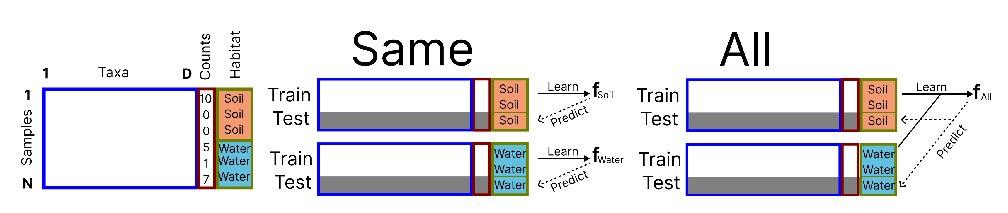
\includegraphics[width=\textwidth]{submission_figures/Fig1.eps}
\caption{Same All Cross-validation (SAC) for microbiome network inference across groups.}
\label{fig:conceptual}
\end{figure}


\subsection{fuser: fused-lasso regularisation}
We implement fused-lasso regularisation using the subgroup-fusion approach proposed by \citet{dondelinger2016hdlss}.
Unlike the ordinary lasso, which only shrinks individual coefficients, the fused-lasso implemented in \texttt{fuser} adds an extra penalty on the pairwise differences between related coefficients, so it enforces both sparsity and smooth (or shared) effects across corresponding coefficients across groups \citep{tibshirani2005fused,dondelinger2016hdlss,fuser2025}.
We model each taxon $d\in\{1,\dots,D\}$ as the response and use the remaining taxa as predictors.
For group
$s\in\{1,\dots,S\}$ and sample $i\in\{1,\dots,n_s\}$ let
\[
y_{i,d}^{(s)} = X_{i,-d}^{(s)} \,\beta_{d}^{(s)} + \varepsilon_{i,d}^{(s)},
\]
where $X_{i,-d}^{(s)}\in\mathbb{R}^{p}$ contains the counts of the
$p=D-1$ predictor taxa. We decompose each group coefficient vector as
\[
\beta_{d}^{(s)} = \beta_{d}^{(0)} + u_{d}^{(s)},
\]
with a global part $\beta_{d}^{(0)}$ shared by all groups and a
deviation $u_{d}^{(s)}$ specific to group $s$.
The parameters are estimated by minimising the objective for each taxon
\[
\begin{aligned}
\mathcal{L}_{d}(\beta_{d}^{(0)},\{u_{d}^{(s)}\}) &= \sum_{s=1}^{S}\sum_{i=1}^{n_s}
  \bigl(y_{i,d}^{(s)} - X_{i,-d}^{(s)}(\beta_{d}^{(0)} + u_{d}^{(s)})\bigr)^{2} \\
&\quad + \lambda\!\Bigl(\lVert\beta_{d}^{(0)}\rVert_{1}
      + \sum_{s=1}^{S}\lVert u_{d}^{(s)}\rVert_{1}\Bigr) \\
&\quad + \gamma\!\sum_{s<t} w_{st}\,
      \lVert u_{d}^{(s)} - u_{d}^{(t)}\rVert_{1},
\end{aligned}
\]
where
% \begin{itemize}
% \item $\lambda > 0$ enforces sparsity of both global and group coefficients (lasso term);
% \item $\gamma \geq 0$ enforces similarity across groups via a \emph{fusion} term (information sharing);
% \item $w_{st}$ are optional non-negative weights encoding a prior graph of group similarity.
% \end{itemize}

\begin{itemize}
  \item $\lambda>0$ enforces sparsity of both global and group coefficients (\emph{lasso} term) \citep{tibshirani2005fused}.
  \item $\gamma\ge 0$ enforces similarity across groups via a \emph{fusion} penalty that shrinks coefficient differences \citep{tibshirani2005fused,dondelinger2016hdlss}.
  \item $w_{st}\!\ge\!0$ are optional weights encoding a prior graph of group similarity \citep{hallac2015network,dondelinger2016hdlss}.
\end{itemize}
In the direct coefficient fusion formulation used in the implementation, $\gamma=0$ reduces the optimisation to separate lasso models, corresponding conceptually to \texttt{glmnet\_same}.
As $\gamma$ increases, coefficients become more similar across groups, approaching a pooled model when the positive fusion weights connect all groups.
Intermediate values allow information sharing while retaining differences between groups.
Exact equivalence to \texttt{glmnet\_same} or \texttt{glmnet\_all} requires matching the remaining modelling choices, including penalty scaling, intercept handling, predictor standardization, and tuning.
The optimisation is repeated for every taxon $d$; final network edges arise from the union of non-zero coefficients across taxa.
Cross-validated grids over $(\lambda,\gamma)$ are used to select the model that minimises prediction test error using Same-All Cross-validation (SAC) for each taxon.

\begin{figure}[t]
\centering
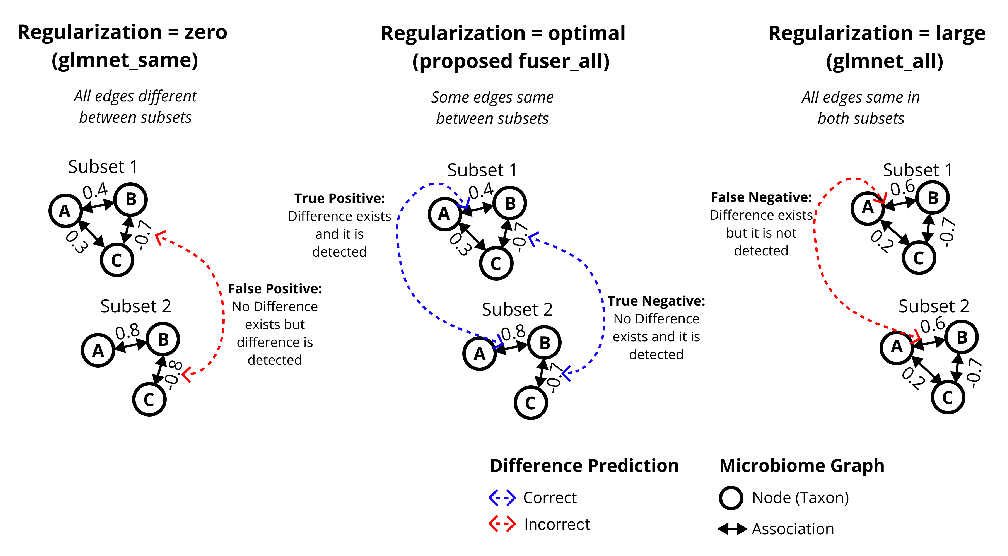
\includegraphics[width=\textwidth]{submission_figures/Fig2.eps}
\caption{Conceptual diagram of regularization for microbiome network inference across groups.}
\label{fig:conceptual2}
\end{figure}

\subsubsection{Regularization Approaches}
Figure~\ref{fig:conceptual2} illustrates the three regularization approaches:
\begin{enumerate}
    \item \textbf{Separate models (\texttt{glmnet\_same}):}
    A model is fit within each group, so corresponding edge weights can differ freely between groups. The lasso sparsity penalty remains, but there is no fusion penalty across groups.
    \item \textbf{Pooled model (\texttt{glmnet\_all}):}
    A single model is fit to training samples pooled across groups, yielding one common set of edge weights.
    \item \textbf{Fused models (\texttt{fuser\_all}):}
    Models for each group are fit jointly, with a fusion penalty encouraging similarity between their coefficients while allowing differences.
\end{enumerate}


\section{Results}
\subsection{Is it better to combine groups?}
Figure~\ref{fig:fuserall_glmnetsame_diff} compares the fused models (\texttt{fuser\_all}) \citep{fuser2025,dondelinger2016hdlss}, trained jointly across groups, with the separate models (\texttt{glmnet\_same}) \citep{friedman2010glmnet}, trained within each group.
These use the All and Same training scenarios, respectively, and are evaluated on excluded samples within each group using SAC \citep{agyapong2025cross, hocking2024soaksameotherallkfoldcrossvalidation}.
The results demonstrate that \texttt{fuser\_all} consistently outperforms \texttt{glmnet\_same} across all datasets, with the magnitude and statistical significance varying by dataset characteristics.
The most substantial improvement occurs in the \textit{TwinsUK} dataset \citep{TwinsUK}, where \texttt{fuser} achieves a mean squared error (MSE) reduction of approximately 0.30 ($p < 0.05$), representing the largest performance gain observed.
For datasets \textit{qa10394} \citep{qa10394}, \textit{HMPv13} \citep{HMP2012}, and \textit{HMPv35} \citep{HMP2012}, \texttt{fuser} shows statistically significant improvements ($p < 0.05$) with MSE reductions ranging from 0.05 to 0.1.
The other datasets, \textit{MovingPictures} \citep{Caporaso2011} and \textit{necromass}, show modest improvements favoring \texttt{fuser} (MSE reductions of approximately 0.02-0.07), but these differences do not reach statistical significance.

\begin{figure}[t]
    \centering
    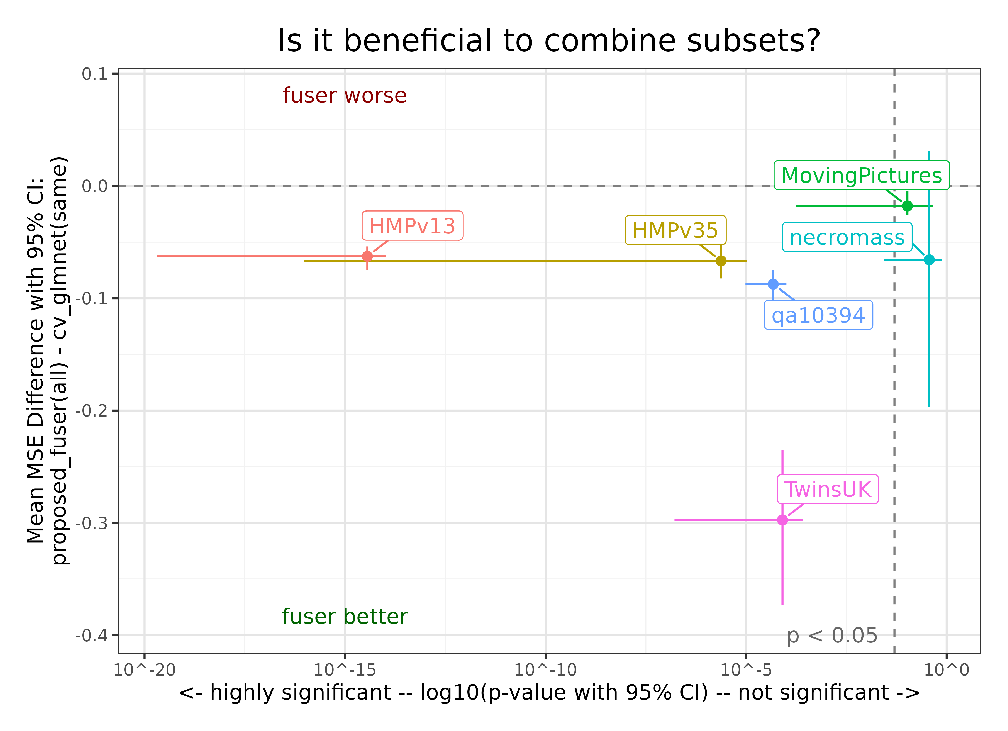
\includegraphics[width=0.85\textwidth]{submission_figures/Fig3.eps}
    \caption{Comparison of \texttt{fuser\_all} and \texttt{glmnet\_same} across datasets.
    Negative mean MSE differences favor \texttt{fuser\_all}.
    The x-axis shows $\log_{10}(p\text{-value})$, with a dashed line at $p = 0.05$.
    Error bars summarize variation across folds.}
    \label{fig:fuserall_glmnetsame_diff}
\end{figure}

\subsection{Do fused models predict better than a pooled model?}
Figure~\ref{fig:fuserall_glmnetall_diff} compares the fused models (\texttt{fuser\_all}) with the pooled model (\texttt{glmnet\_all}); both use training samples from all groups.
The results demonstrate that \texttt{fuser\_all} consistently outperforms \texttt{glmnet\_all} across all datasets when both methods utilize all available groups.
All six datasets show improved performance favoring \texttt{fuser}, with mean squared error reductions ranging from near-zero to approximately 0.10.
Three datasets, \textit{TwinsUK} \citep{TwinsUK}, \textit{qa10394} \citep{qa10394}, and \textit{HMPv13} \citep{HMP2012}, achieve statistically significant improvements ($p < 0.05$), with \textit{TwinsUK} \citep{TwinsUK} showing the most substantial performance gain.
The \textit{necromass} dataset shows a notable improvement that approaches but does not reach statistical significance.

\begin{figure}[t]
    \centering
    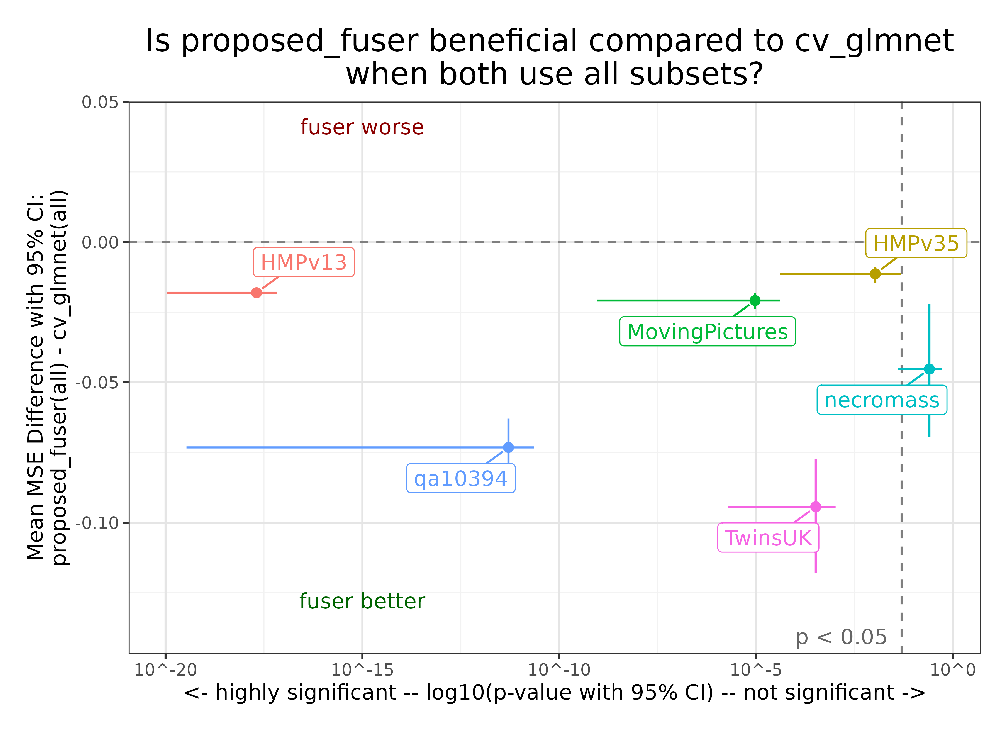
\includegraphics[width=0.85\textwidth]{submission_figures/Fig4.eps}
    \caption{Comparison of \texttt{fuser\_all} and \texttt{glmnet\_all} across datasets.
    Negative mean MSE differences favor \texttt{fuser\_all}.
    The x-axis shows $\log_{10}(p\text{-value})$, with a dashed line at $p = 0.05$.
    Error bars summarize variation across folds.}
    \label{fig:fuserall_glmnetall_diff}
\end{figure}


\subsection{Performance for individual taxa reveals algorithm complementarity}
While analyses on the dataset level demonstrate overall trends, examining individual taxon reveals substantial heterogeneity in optimal regularization strategies across microbial species.
Figure~\ref{fig:taxa_performance_movingpictures} illustrates this pattern using representative taxa from the \textit{MovingPictures} dataset, where different taxa exhibit distinct preferences for regularization approaches.
The results demonstrate that no single algorithm universally outperforms others across all taxa within a dataset.
For example, Taxa4383166 achieves lowest prediction error with \texttt{glmnet\_same} ($p < 0.01$), suggesting this taxon benefits from separate modeling within each group without information sharing.
In contrast, Taxa4450795 shows significantly improved performance with \texttt{fuser\_all} ($p < 0.01$), indicating this taxon's associations are enhanced by fusion-based regularization across environmental niches.
Taxa4467447 performs optimally under \texttt{glmnet\_all}, suggesting its associations are consistent across environments and benefit from increased sample size without specialized regularization.
Taxa with conserved ecological roles across environments may benefit from standard regularization with larger sample sizes, while environmentally responsive taxa may require fusion-based approaches to capture association patterns within each group \citep{fuser2025,dondelinger2016hdlss}.

\begin{figure}[t]
    \centering
    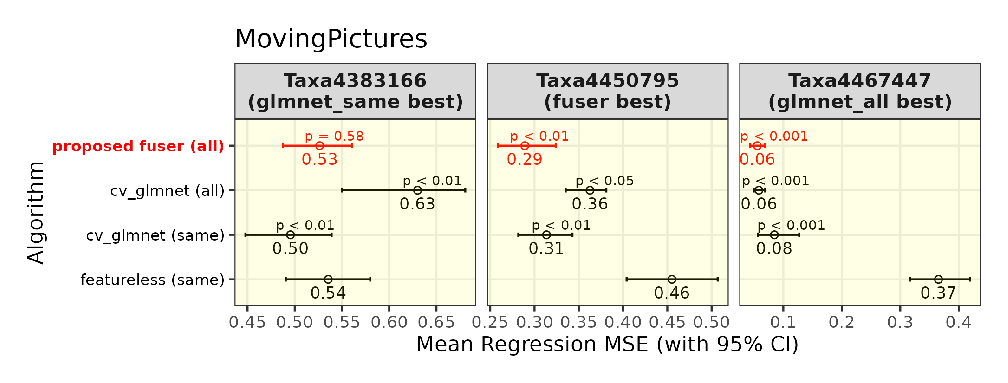
\includegraphics[width=0.85\textwidth]{submission_figures/Fig5.eps}
    \caption{Prediction performance for three taxa in MovingPictures.
    Taxa4383166 favors \texttt{glmnet\_same}, Taxa4450795 favors \texttt{fuser\_all}, and Taxa4467447 favors \texttt{glmnet\_all}.}
    \label{fig:taxa_performance_movingpictures}
\end{figure}

\subsection{Model comparison after centered log ratio transformation}
To examine whether our model comparisons were sensitive to compositional preprocessing, we repeated the analysis using a target exempt version (to prevent data leakage) of the centered log ratio transformation in MovingPictures, necromass, and TwinsUK.
For each target taxon, we calculated the mean logged abundance of the remaining taxa within each sample and subtracted this reference from both the target and the predictors.
Excluding the target from the reference prevents its observed abundance from entering the predictor transformation.
We retained the model comparisons and cross validation framework used in the original analysis.

Figure~\ref{fig:clr_sensitivity} shows that the results varied across datasets and comparison methods.
In MovingPictures, most taxa had lower prediction error with \texttt{fuser\_all} than with either glmnet approach.
In necromass, the median differences favored \texttt{fuser\_all} in both comparisons, although some taxa favored glmnet.
In TwinsUK, most taxa favored \texttt{fuser\_all} over \texttt{glmnet\_same}, while differences between \texttt{fuser\_all} and \texttt{glmnet\_all} were centered near zero.
The benefit of sharing information across groups was broadly maintained after the target exempt log ratio transformation. 
However, the advantage of fusion over a single pooled model depended on the dataset and preprocessing.

\begin{figure}[t]
    \centering
    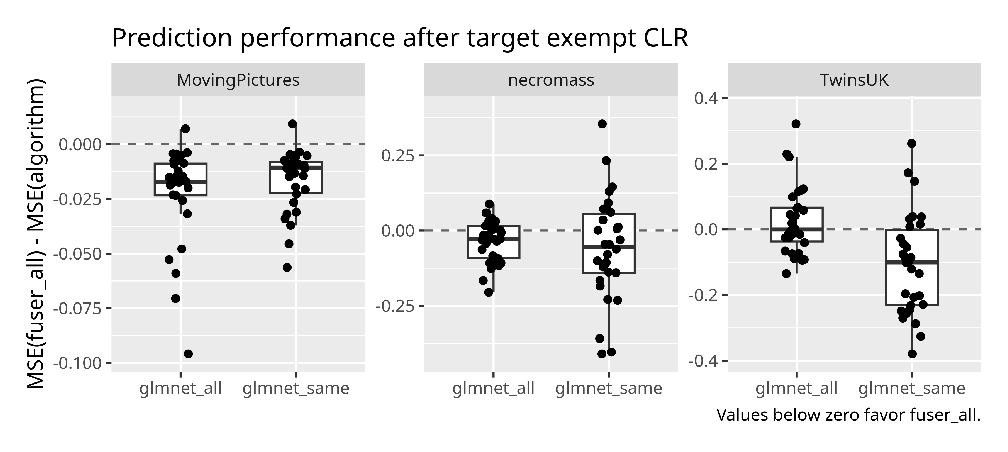
\includegraphics[width=\textwidth]{submission_figures/Fig6.eps}
    \caption{\textbf{Prediction performance after a target exempt log ratio transformation.}
    Each point represents one taxon's mean test MSE difference across folds and test groups.
    Negative values favor \texttt{fuser\_all}.}
    \label{fig:clr_sensitivity}
\end{figure}


\section{Discussion and Conclusion}
\subsection{Necromass microbial community difference networks}
In this analysis, we focused on comparing two distinct treatment groups from our experimental design: AllSoilM1M3 (soil samples from both Month 1 and Month 3 timepoints) and LowMelM1 (low melanization necromass samples from Month 1 timepoint). 
These two groups were selected to examine the fundamental differences between soil and necromass microbial communities while controlling for melanization level and minimizing temporal variation effects.
Figure~\ref{fig:necromass_networks} illustrates how different regularization strategies affect the detection of edge weight differences across groups in the necromass microbial real data.
In these difference networks, an edge between taxa indicates a difference in association strength between groups, while absence of an edge signifies consistency across groups.

\begin{figure}[t]
\centering
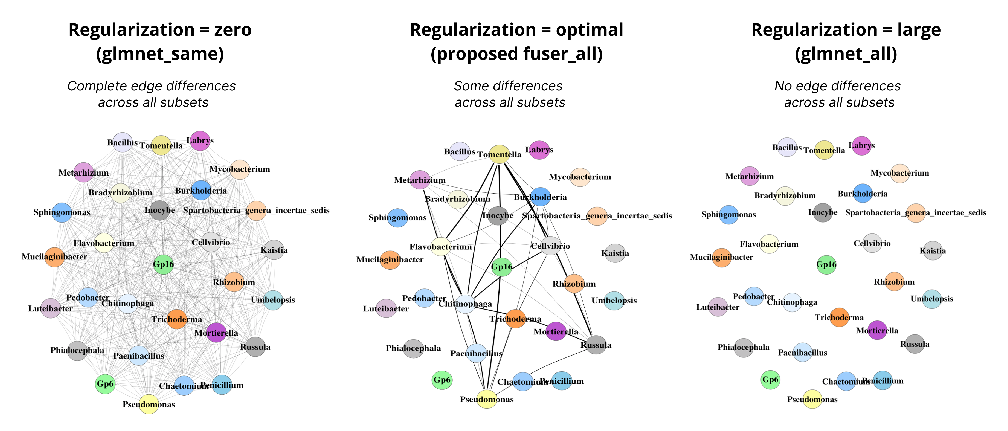
\includegraphics[width=\textwidth]{submission_figures/Fig7.eps}
\caption{\textbf{Impact of regularization on detected edge weight differences in the necromass microbial community.}
Node positions are preserved across panels, with each node representing a taxon.
Edges indicate detected differences in association strength between groups, with edge weights reflecting the magnitude of difference.
No edges indicate consistent associations across groups.
}
\label{fig:necromass_networks}
\end{figure}

Separate models (\texttt{glmnet\_same}) produce a dense, fully connected difference network.
A pooled model (\texttt{glmnet\_all}) uses common microbial association coefficients across groups, resulting in a fully sparse difference network where no edges are detected.
The fused models (\texttt{fuser\_all}) produce a difference network with intermediate density, allowing some coefficients to differ across groups while others are shared.
However, the fused models (\texttt{fuser\_all}) do not always predict better than the pooled model (\texttt{glmnet\_all}), even though both use training samples from all groups.

\subsection{Conclusion}
Fusion improved predictive performance in our comparisons, although its advantage over pooling depended on the dataset and preprocessing.
While our approach significantly improves cross-environment inference, several limitations should be acknowledged \citep{dohlman2019interactome}.
The optimal regularization parameters remain data-driven, requiring careful cross-validation for each application which is computationally intensive \citep{hocking2024soaksameotherallkfoldcrossvalidation, agyapong2025cross}.
While \texttt{fuser} captures differences between groups, it may not fully account for phylogenetic relationships or functional potentials of taxa, which could further refine ecological interpretations \citep{liu2024phylo,kunin2005phylogenetic,Douglas2020}.
The algorithm's performance is contingent on the quality and representativeness of the input abundance data, which can vary widely across microbiome studies \citep{Sinha2017,McLaren2019,Gibbons2018}.
The observed abundance tables are also compositional because each sample is constrained by its sequencing depth. 
Log transformation does not remove this constraint, and some estimated associations may reflect compositional effects. 
All methods in our comparison use the same preprocessing, so held-out prediction error provides a common measure of model generalization. 
However, lower prediction error does not show that the estimated network is the biological ground-truth network and validating individual edges are outside the scope of this study.
Despite these limitations, our results demonstrate that \texttt{fuser} provides a robust framework for microbial network inference across groups, effectively balancing the trade-offs between overfitting and underfitting.
Future work should explore the application of this SAC technique to incorporate phylogenetic information and metabolic potentials to further refine our understanding of when and why microbial associations differ across environments \citep{liu2024phylo,dohlman2019interactome}.


\section*{Acknowledgments}
The authors would like to thank F. Maillard for oversight in generating the necromass dataset as well as the Microbes Persist Soil Microbiome SFA Award SCW1632 from the U.S. Department of Energy, Office of Biological and Environmental Research, Genomic Science Program, which facilitated this research collaboration.

\section*{Author Contributions}
\textbf{Daniel Agyapong:} Conceptualization, Methodology, Software, Formal analysis, Writing - original draft.
\textbf{Briana H. Beatty:} Data curation, Resources (generated necromass dataset).
\textbf{Peter G. Kennedy:} Validation, Writing - review \& editing.
\textbf{Jane C. Marks:} Validation, Writing - review \& editing.
\textbf{Toby D. Hocking:} Methodology, Algorithm design, Supervision, Writing - review \& editing.

\section*{Statements and Declarations}
\subsection*{Ethical considerations}
This study used publicly available microbiome datasets. No new human participants were recruited, and ethical approval was not required for this secondary analysis.

\subsection*{Consent to participate}
No participants were recruited for this secondary analysis of publicly available data.

\subsection*{Consent for publication}
No identifying information about individual participants is reported.

\subsection*{Declaration of conflicting interest}
The authors declare that they have no known competing financial interests or personal relationships that could have appeared to influence the work reported in this paper.

\subsection*{Data and Software Availability}
The data and code used in this study are publicly available at \url{https://github.com/EngineerDanny/necromass}.

\subsection*{Funding}
This work was funded by the National Science Foundation grant \#2125088 from Rules of Life Program.


%% --- BIBLIOGRAPHY ---

\bibliographystyle{sageh}
\bibliography{references}

\end{document}
